\documentclass{article} % This line defines the type of document. 'article' is a common class for small documents.
\usepackage[margin=1in]{geometry}
\usepackage{graphicx}
\usepackage{titlesec}

\titleformat{\section}
  {\normalfont\large\bfseries}{\thesection}{1em}{}

\begin{document} % This line marks the beginning of the document content.


\noindent\makebox[\linewidth]{\rule{\textwidth}{1pt}} 
\vspace*{0mm} % adds vertical space before the title
\begin{center}
    \Large\textbf{Toy Models of Superposition Replication and Findings}
\end{center}
\vspace*{2mm} % adds vertical space before the title
\noindent\makebox[\linewidth]{\rule{\textwidth}{1pt}}
\newline

\begin{abstract}
\begin{quote}
    Toy Models of Superpostion\cite{elhage2022toy} is a groundbreaking paper published by 
    researchers affilated with Anthropic and Harvard University in 2022. The
    paper demonstrates that neural networks can represent more features than
    they have demensions buy training small models with under 100 neurons. Additionally,
    they use these so called "toy models" to understand the relationship between
    how neural networks are trained and how they represent the data internally.
    This paper was able to the finding from this paper and make new observations
    about "toy models" and how they behave under different training circumstances.
\end{quote}
\end{abstract}


\section{Introduction}


\begin{figure}[h]
    \centering
    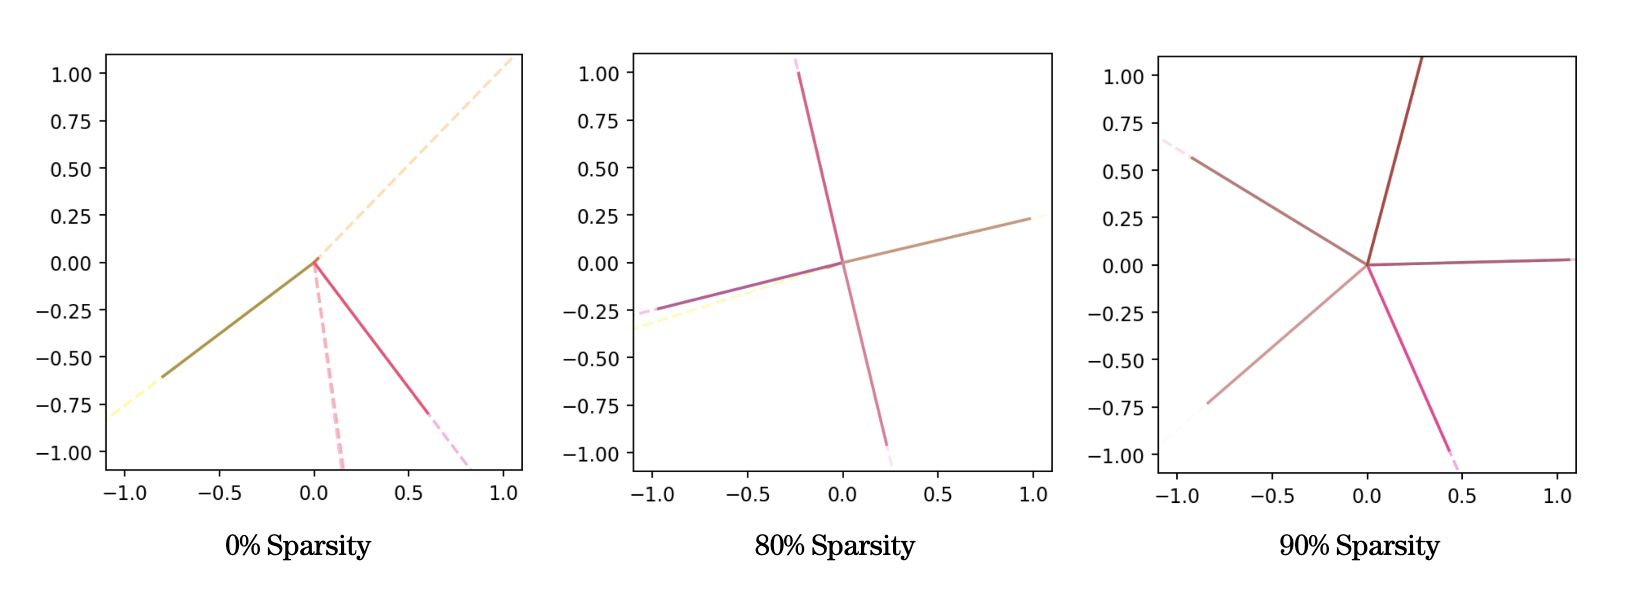
\includegraphics[width=0.7\linewidth]{section_1/images/section1_replicated_graphic.png}
    \caption{Replicated feature directions example.}
    \label{fig:section1_replication}
\end{figure}

\begin{figure}[h]
    \centering
    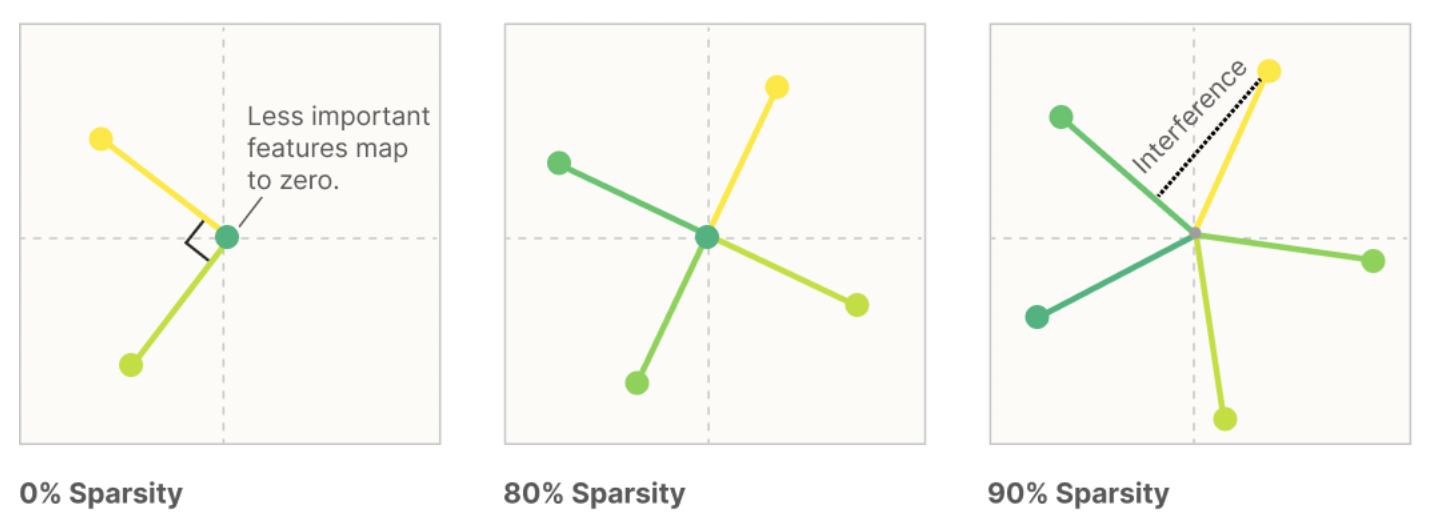
\includegraphics[width=0.67\linewidth]{section_1/images/section1_anthropic_graphic_.png}
    \caption{Graphic from Anthropic Paper}
    \label{fig:section1_anthropic}
\end{figure}

\bibliographystyle{plain}
\bibliography{references}

\end{document} % This line marks the end of the document content.
